% !TEX TS-program = xelatex
\documentclass[aspectratio=169]{beamer}

% --- THEME & LAYOUT ---
\usetheme[numbering=fraction,progressbar=head]{metropolis}
\setbeamersize{text margin left=8mm,text margin right=8mm}

% --- CUSTOM FOOTER WITH TLP MARKING ---
\setbeamertemplate{frame footer}{\textbf{TLP:CLEAR} — Information may be shared freely without restriction.}
\setbeamercolor{frame footer}{fg=cyber-accent}

% --- FONTS (XeLaTeX) ---
\usepackage{fontspec}
\setsansfont[
  Ligatures=TeX, Scale=1.02,
  BoldFont = {IBM Plex Sans Bold},
  ItalicFont = {IBM Plex Sans Italic}
]{IBM Plex Sans}
\setmonofont{IBM Plex Mono}

% --- ICONS ---
\usepackage{fontawesome5}

% --- COLORS (cyber palette) ---
\definecolor{cyber-bg}{HTML}{0B0F14}
\definecolor{cyber-ink}{HTML}{E6EEF5}
\definecolor{cyber-accent}{HTML}{217EAA}
\definecolor{cyber-mid}{HTML}{7D9CB7}
\definecolor{cyber-soft}{HTML}{8CA4AC}
\setbeamercolor{normal text}{fg=cyber-ink,bg=cyber-bg}
\setbeamercolor{frametitle}{fg=cyber-ink,bg=cyber-bg}
\setbeamercolor{progress bar}{fg=cyber-accent,bg=cyber-soft}
\setbeamercolor{alerted text}{fg=cyber-accent}

% --- LINKS ---
\hypersetup{colorlinks=true, linkcolor=cyber-accent, urlcolor=cyber-accent}

% --- CODE / BOXES ---
\usepackage{listings}
\lstset{
  basicstyle=\ttfamily\footnotesize,
  backgroundcolor=\color{black!5},
  frame=single, rulecolor=\color{cyber-soft},
  keywordstyle=\color{cyber-accent}\bfseries,
  commentstyle=\color{cyber-soft},
  showstringspaces=false
}
\usepackage[most]{tcolorbox}
\tcbset{colback=black!5!cyber-bg, colframe=cyber-soft, coltext=cyber-ink, boxsep=1mm, left=2mm, right=2mm}

% --- GRAPHICS ---
\usepackage{graphicx}

% --- SPEAKER NOTES ---
\usepackage{pgfpages}
% \setbeameroption{hide notes}
% \setbeameroption{show notes}
% \setbeameroption{show only notes}

% --- TITLE INFO ---
\title{\faIcon{shield-alt}\; Range42 — Semi-Technical Overview}
\subtitle{Modular Cyber Range Platform for Real-World Readiness}
\author{NC3 / Range42 Team}
\date{\today}
\institute{\faServer\; Proxmox \quad \faCogs\; Ansible \quad \faProjectDiagram\; Orchestration \quad \faBinoculars\; Telemetry}

\begin{document}

% --- TITLE ---
\begin{frame}
  \titlepage
  \note[item]{Goal: 20-minute semi-technical tour of Range42's building blocks and roadmap.}
  \note[item]{Audience: technical staff who aren't deep specialists.}
\end{frame}

% --- PUBLIC MONEY PUBLIC CODE ---
\begin{frame}{Public money, public code. Let's go all the way, shall we?}
  \begin{columns}[T]
    \column{0.65\textwidth}
    \textbf{Current Team}
    \begin{itemize}
      \item Core development team of 3-5 contributors
      \item Mix of security researchers, DevOps engineers, and platform architects
      \item Collaborative model with NC3 and academic partners
    \end{itemize}
    
    \textbf{Current Funding}
    \begin{itemize}
      \item Public sector grant funding for cyber training infrastructure
      \item Open-source model: no licensing fees, transparent development
      \item Investment in reusable, community-owned tooling
    \end{itemize}
    
    \textbf{Current Challenges}
    \begin{itemize}
      \item Governance standardization across 13+ repositories
      \item Balancing rapid development with documentation maturity
      \item Sustainable maintenance model as project scales
    \end{itemize}
    
    \column{0.3\textwidth}
    \vspace{10mm}
    \begin{figure}
      \centering
      
\includegraphics[width=\textwidth]{images/logos/FSFE_Public_Money_Public_Code_logo.pdf}
    \end{figure}
  \end{columns}
  \note[item]{Emphasize public funding → public ownership → public benefit.}
  \note[item]{Range42 embodies PMPC principles: taxpayer-funded development results in freely available, auditable infrastructure.}
\end{frame}

% --- AGENDA ---
\begin{frame}{Agenda}
  \begin{enumerate}
    \item What Range42 is \& why it matters
    \item Competitive landscape
    \item Architecture at a glance
    \item Repository audit findings (13 repositories analyzed)
    \item Risks, governance, and quality gates
    \item 90-day roadmap \& demo plan
  \end{enumerate}
  \note[item]{Keep flow brisk; ~2–3 min per major section.}
\end{frame}

% --- WHAT IS RANGE42 ---
\begin{frame}{What is Range42?}
  \begin{itemize}
    \item \textbf{Modular cyber range platform} for offensive, defensive, and hybrid training.
    \item \textbf{Reproducible IaC}: build, deploy, document labs via Proxmox, Ansible, Docker.
    \item \textbf{Private APIs} for orchestration \& telemetry; developer toolkits for pipelines.
  \end{itemize}
  \begin{tcolorbox}
    \faInfoCircle\; Built to simulate \emph{real-world incidents} safely, with isolation, snapshots, and telemetry.
  \end{tcolorbox}
  \note[item]{Anchor on "safe realism": isolation, resets, data trails.}
\end{frame}

% --- COMPETITIVE LANDSCAPE ---
\begin{frame}{Range42 vs. Other Cyber Ranges}
  \begin{table}
    \scriptsize
    \begin{tabular}{l|cccc}
      \textbf{Feature} & \textbf{Range42} & \textbf{Commercial SaaS} & \textbf{Cloud Native} & \textbf{Traditional} \\
      \hline
      \alert{Open Architecture} & \checkmark & \texttimes & \texttimes & \texttimes \\
      \alert{IaC/GitOps} & \checkmark & \textasciitilde & \checkmark & \texttimes \\
      Private Deployment & \checkmark & \texttimes & \textasciitilde & \checkmark \\
      Cost Control & \checkmark & \texttimes & \textasciitilde & \checkmark \\
      Full Data Custody & \checkmark & \texttimes & \texttimes & \checkmark \\
      API Orchestration & \checkmark & \checkmark & \checkmark & \texttimes \\
      Rapid Reset/Snapshots & \checkmark & \checkmark & \textasciitilde & \textasciitilde \\
      Custom Scenarios & \checkmark & \texttimes & \textasciitilde & \checkmark \\
    \end{tabular}
  \end{table}
  \vspace{2mm}
  \begin{tcolorbox}
    \faLightbulb\; \textbf{Range42's Edge}: Full control, reproducibility, and cost-effectiveness without vendor lock-in.
  \end{tcolorbox}
  \note[item]{Emphasize open architecture and IaC as key differentiators.}
  \note[item]{Commercial SaaS: SimSpace, Immersive Labs, RangeForce, Cyberbit.}
\end{frame}

% --- ARCH OVERVIEW ---
\begin{frame}{Architecture at a Glance}
  \begin{itemize}
    \item \textbf{Hypervisor layer}: Proxmox VMs/LXCs; snapshots; network segments.
    \item \textbf{Automation layer}: Ansible roles orchestrate lifecycle, network, firewall, images.
    \item \textbf{Control plane}: Backend API (routes for VM/Net/Runner); Kong gateway.
    \item \textbf{UX}: Deployer UI (visual design), EMP mockup (exercise mgmt), trainee access.
    \item \textbf{Observability}: Wazuh for logs/alerts; structured telemetry.
  \end{itemize}
  \note[item]{Emphasize modularity: builder/deployer/runner + gateway.}
\end{frame}

\begin{frame}{Architecture: Logical Components → Repository Mapping}
  \begin{figure}
    \centering
    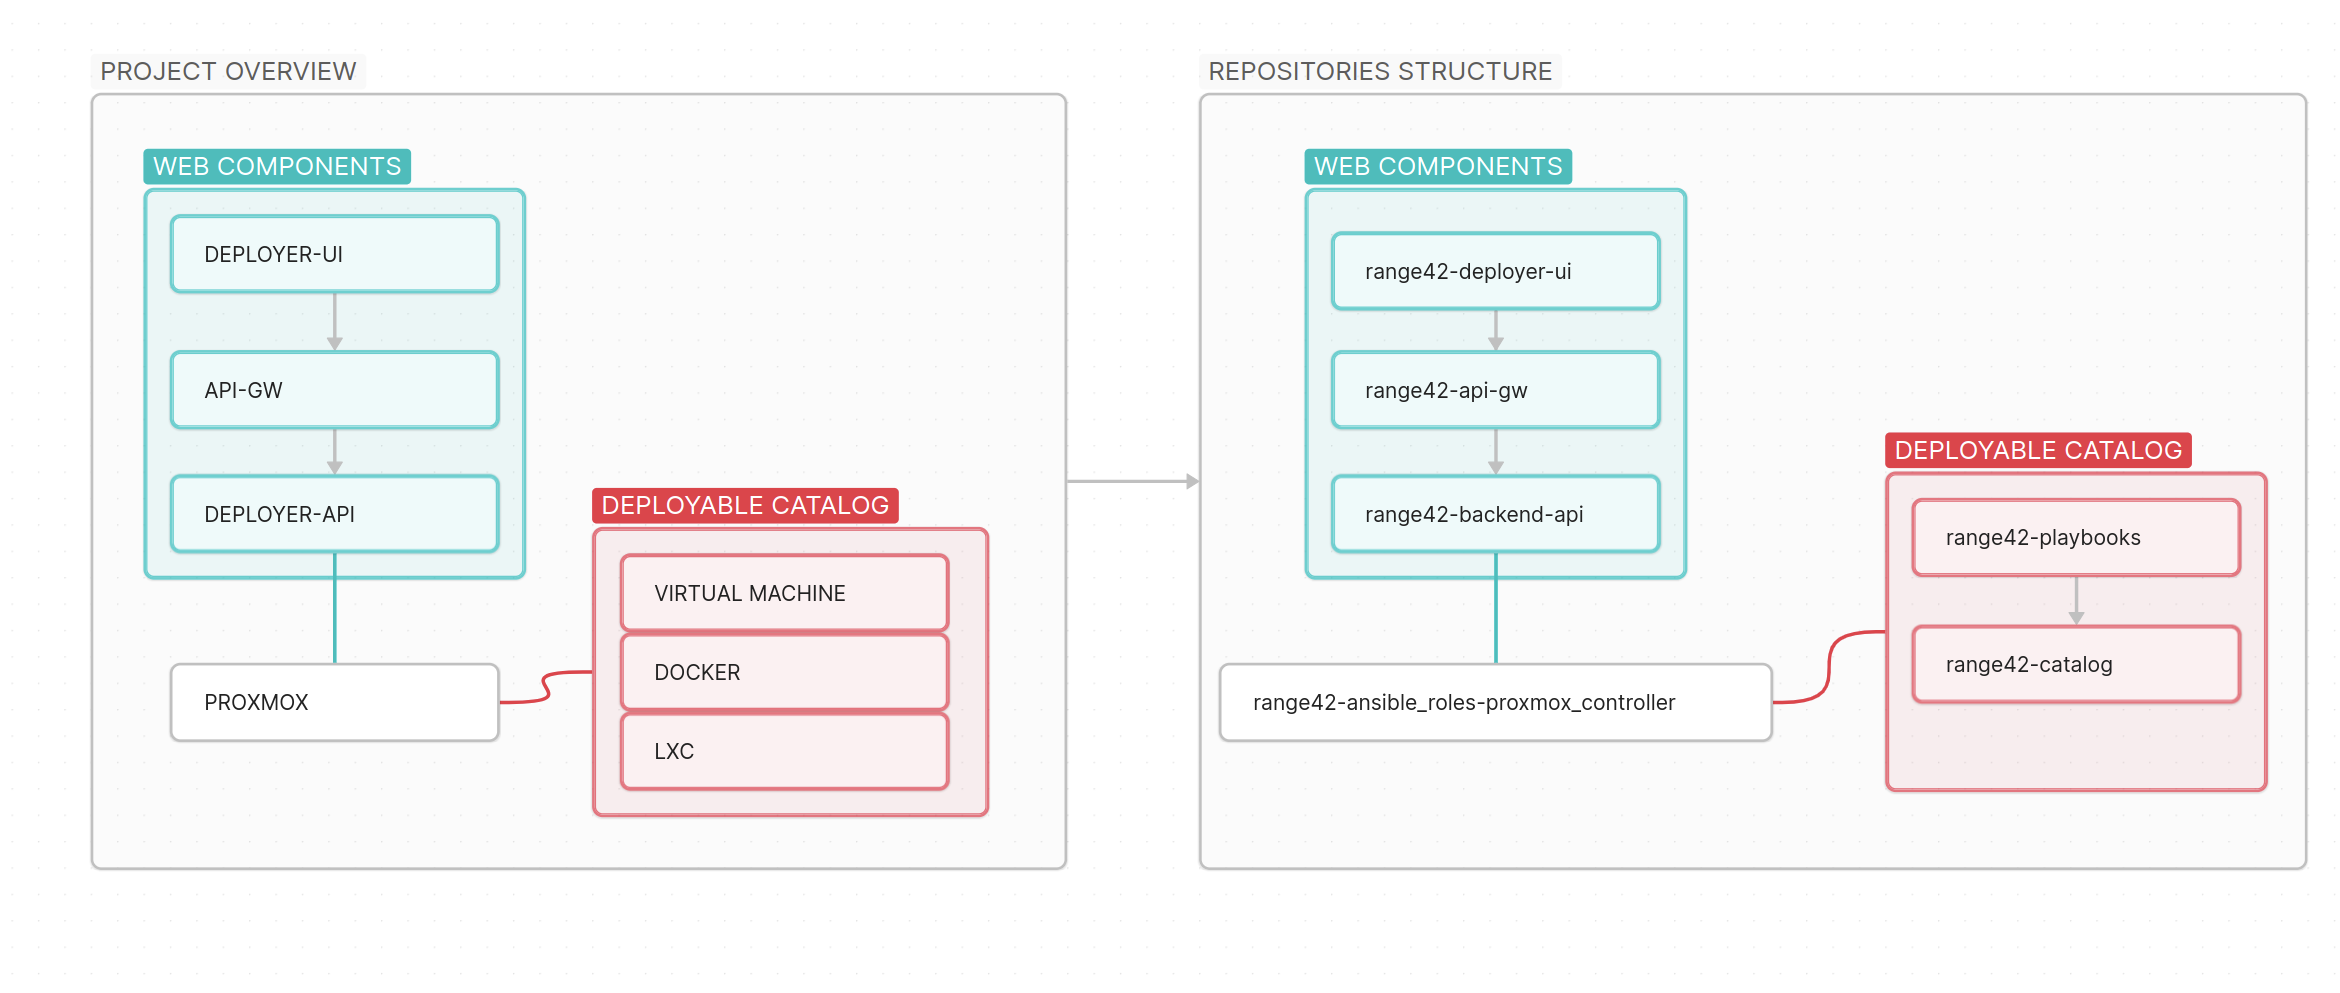
\includegraphics[width=0.95\textwidth]{images/diagrams/architecture.png}
  \end{figure}
  \vspace{-2mm}
  \begin{tcolorbox}
    \faInfoCircle\; \textbf{Left}: Logical architecture flow. \textbf{Right}: Actual GitHub repository structure.
  \end{tcolorbox}
  \note[item]{Left side shows logical architecture; right side shows actual GitHub repos.}
  \note[item]{Emphasize how web components flow through API gateway to backend, which controls Proxmox via Ansible role.}
  \note[item]{Deployable catalog (playbooks + catalog repos) contains the infrastructure-as-code content.}
\end{frame}

% === REPOSITORY AUDIT OVERVIEW ===
\section{Repository Audit Findings}

\begin{frame}{Organization-Wide Audit Results \; \faClipboardCheck}
  \textbf{13 Repositories Analyzed} (2 public, 11 private)\\[3mm]
  
  \textbf{Critical Findings}
  \begin{itemize}
    \item \alert{9/13 repositories} have LICENSE template placeholders (\texttt{<year>}, \texttt{<name of author>})
    \item \alert{13/13 repositories} missing SECURITY.md vulnerability disclosure policy
    \item \alert{12/13 repositories} have no CI/CD pipeline
    \item \alert{0 repositories} have all required governance files
  \end{itemize}
  \vspace{2mm}
  \begin{tcolorbox}
    \faCheckCircle\; \textbf{Good News}: Zero high-severity security findings across all code scans (bandit, pip-audit, npm audit).
  \end{tcolorbox}
  \note[item]{Sanity check performed 2025-09-30 using gh-repo-organizer tool.}
  \note[item]{Security posture is excellent; governance is the primary gap.}
\end{frame}

% === AUTOMATION LAYER ===
\section{Automation}

\begin{frame}{range42-ansible\_roles-private-devkit \; \faTerminal}
  \textbf{Status:} Active \hfill \textbf{Commits:} 179 \hfill \textbf{Lang:} Shell\\[2mm]
  \textbf{Purpose:} Helper scripts for Proxmox and Ansible operations including VM/LXC management, firewall rules, and JSON transformations.\\[2mm]
  \textbf{Key Findings}
  \begin{itemize}
    \item DevKit provides 100+ helper scripts following strict naming convention for Proxmox automation.
    \item Zero Bandit findings; actively used with 179 commits but lacks CI pipeline.
    \item Critical need: finalize LICENSE placeholders and add governance documentation for contributors.
  \end{itemize}
  \note[item]{Mature and heavily used repository with excellent naming conventions.}
  \note[item]{Top priority is adding CI with shellcheck/shfmt and completing governance files to enable safe community contributions.}
\end{frame}

\begin{frame}{range42-ansible\_roles-proxmox\_controller \; \faCogs}
  \textbf{Status:} Active \hfill \textbf{Commits:} 108 \hfill \textbf{Lang:} Ansible/YAML\\[2mm]
  \textbf{Purpose:} Ansible role for managing Proxmox nodes via API: VMs, LXC containers, networking, storage, firewall, and snapshots.\\[2mm]
  \textbf{Key Findings}
  \begin{itemize}
    \item Comprehensive Ansible role managing full Proxmox lifecycle via API with 108 commits.
    \item Broad functionality coverage but lacks CI pipeline for ansible-lint and idempotence tests.
    \item Immediate actions: finalize LICENSE, add CI, and document variables with example playbooks.
  \end{itemize}
  \note[item]{Core infrastructure role with strong breadth.}
  \note[item]{Needs production hardening through CI with ansible-lint and Molecule, plus improved onboarding documentation for variable definitions and usage examples.}
\end{frame}

% === CONTROL PLANE ===
\section{Control Plane}

\begin{frame}{range42-backend-api \; \faProjectDiagram}
  \textbf{Status:} Active \hfill \textbf{Commits:} 125 \hfill \textbf{Lang:} Python/Shell/YAML\\[2mm]
  \textbf{Purpose:} FastAPI backend orchestrating Proxmox deployments via Ansible, with routes for VM control, networking, and bundle execution.\\[2mm]
  \textbf{Security/Quality}
  \begin{itemize}
    \item FastAPI backend with 125 commits; clean security scans (bandit, pip-audit, safety).
    \item Comprehensive route structure for Proxmox control and bundle orchestration via Ansible.
    \item Production hardening needed: add CI pipeline, unit tests, finalize LICENSE, and SECURITY policy.
  \end{itemize}
  \note[item]{Well-structured backend with excellent security posture.}
  \note[item]{Priority actions are adding CI with pytest, formalizing API contracts with the definitions repo, and completing governance documentation.}
\end{frame}

\begin{frame}{range42-api-definitions \; \faSitemap}
  \textbf{Status:} Stale \hfill \textbf{Commits:} 5 \hfill \textbf{Lang:} JSON\\[2mm]
  \textbf{Purpose:} Placeholder repository for OpenAPI/Swagger specifications defining the Range42 backend API contracts.\\[2mm]
  \textbf{Decision Point}
  \begin{itemize}
    \item Placeholder repository with OpenAPI specs but minimal content and only 5 commits.
    \item Missing LICENSE file entirely; needs decision on archive versus active development.
    \item If kept: seed with comprehensive API definitions and add CI for spec validation.
  \end{itemize}
  \note[item]{Decision point repository: either archive to reduce noise or commit to making it the single source of API truth with comprehensive OpenAPI specs and validation tooling.}
\end{frame}

\begin{frame}{range42-api-gw \; \faIcon{shield-alt}}
  \textbf{Status:} Active \hfill \textbf{Commits:} 5 \hfill \textbf{Lang:} N/A\\[2mm]
  \textbf{Purpose:} Kong API Gateway configuration for authentication, ACL, and access control policies in front of backend API.\\[2mm]
  \textbf{Key Findings}
  \begin{itemize}
    \item Kong API Gateway repository for authentication and access control with minimal current content.
    \item LICENSE has template placeholders; needs Kong declarative configs or deployment manifests.
    \item Add documentation for Kong setup, plugin configuration, and integration with backend API.
  \end{itemize}
  \note[item]{Early-stage repository that needs Kong configuration files, deployment guides, and completed governance files.}
  \note[item]{Critical for production security but currently underdeveloped.}
\end{frame}

% === UX LAYERS ===
\section{UX Layers}

\begin{frame}{range42-deployer-ui \; \faDrawPolygon}
  \textbf{Status:} Prototype \hfill \textbf{Commits:} 28 \hfill \textbf{Lang:} Vue/TS\\[2mm]
  \textbf{Purpose:} VueFlow-based visual orchestrator for designing, validating, and deploying Range42 infrastructure through node-based interface.\\[2mm]
  \textbf{Key Findings}
  \begin{itemize}
    \item VueFlow-based UI with node-based infrastructure design; unit/e2e tests exist but no CI.
    \item Good UX foundation with i18n support and localStorage data management for offline capability.
    \item Wire CI for automated testing, stabilize API contracts with backend, and resolve npm advisory.
  \end{itemize}
  \note[item]{Promising prototype with solid testing foundation.}
  \note[item]{Key next steps are enabling CI to run existing tests, hardening API contract validation, and improving export/import error handling.}
\end{frame}

\begin{frame}{range42-emp-mockup \; \faChalkboardTeacher}
  \textbf{Status:} Prototype \hfill \textbf{Commits:} 1 \hfill \textbf{Lang:} Vue/TS\\[2mm]
  \textbf{Purpose:} Exercise Management Platform scaffold with basic Vue 3 routing, TypeScript setup, and unit test foundation.\\[2mm]
  \textbf{Key Findings}
  \begin{itemize}
    \item Exercise Management Platform seed project with 1 commit; basic Vue 3 scaffold only.
    \item Missing LICENSE entirely; has 2 low npm advisories and no CI pipeline.
    \item Define MVP scope and architecture first, then add CI and resolve dependency vulnerabilities.
  \end{itemize}
  \note[item]{Very early prototype requiring architectural definition before development continues.}
  \note[item]{Must add LICENSE, resolve npm advisories, and establish CI pipeline once MVP scope is clear.}
\end{frame}

% === INFRASTRUCTURE & CONTENT ===
\section{Infrastructure \& Content}

\begin{frame}{range42-playbooks \; \faCubes}
  \textbf{Status:} Active \hfill \textbf{Commits:} 75 \hfill \textbf{Lang:} Ansible/YAML\\[2mm]
  \textbf{Purpose:} Centralized Ansible playbooks organizing scenarios and bundles for CLI or backend API orchestration of infrastructure deployments.\\[2mm]
  \textbf{Key Findings}
  \begin{itemize}
    \item Central playbook repository with 75 commits organizing scenarios and reusable bundles.
    \item Clear structure with test scripts but no CI for ansible-lint or syntax validation.
    \item Add CI pipeline, introduce scenario taxonomy with tags, and document compatibility matrices.
  \end{itemize}
  \note[item]{Well-organized orchestration layer with good separation between scenarios and bundles.}
  \note[item]{Needs CI enforcement for ansible-lint and comprehensive documentation of scenario dependencies and compatibility.}
\end{frame}

\begin{frame}{range42-catalog \; \faBoxes}
  \textbf{Status:} Active \hfill \textbf{Commits:} 91 \hfill \textbf{Lang:} Ansible/YAML\\[2mm]
  \textbf{Purpose:} Collection of reusable Ansible roles and Docker/Compose stacks for deploying vulnerable scenarios and infrastructure bundles.\\[2mm]
  \textbf{Key Findings}
  \begin{itemize}
    \item Catalog of Ansible roles and Docker stacks for deploying training scenarios with 91 commits.
    \item Volatile tree structure organizing CVEs and misconfigurations by technology type.
    \item Add CI for ansible-lint, introduce scenario taxonomy with tags, and finalize LICENSE.
  \end{itemize}
  \note[item]{Cornerstone content repository that needs structural stabilization, metadata standardization with scenario tags, and CI pipeline to prevent drift as content grows.}
\end{frame}

% === DOCUMENTATION & GOVERNANCE ===
\section{Documentation \& Governance}

\begin{frame}{.github — Community Health Files \; \faUsers}
  \textbf{Status:} Active \hfill \textbf{Commits:} 13 \hfill \textbf{Lang:} Markdown/YAML\\[2mm]
  \textbf{Purpose:} Organization-wide default community health files to standardize CODE\_OF\_CONDUCT, CONTRIBUTING, SECURITY, issue/PR templates, and support docs across public repositories.\\[2mm]
  \textbf{Key Findings}
  \begin{itemize}
    \item Centralizes community health files for all public repos.
    \item Add CI to lint templates and validate YAML.
    \item Document private-repo strategy and license requirements.
  \end{itemize}
  \begin{tcolorbox}
    \faExclamationTriangle\; \textbf{Critical Limitation}: Defaults apply \emph{only} to public repos; private repos need local copies. LICENSE files cannot be inherited—each repo must add its own.
  \end{tcolorbox}
  \note[item]{This repo ensures consistent governance and contribution hygiene across Range42 public projects.}
  \note[item]{Note that LICENSE files are per-repo and private repos won't inherit defaults; add CI to catch template regressions.}
\end{frame}

\begin{frame}{range42-documentation-private-obsidian \; \faBook}
  \textbf{Status:} Active \hfill \textbf{Commits:} 3 \hfill \textbf{Lang:} Markdown/Shell\\[2mm]
  \textbf{Purpose:} Private Obsidian vault containing architecture canvases, meeting notes, API drafts, and internal documentation.\\[2mm]
  \textbf{Key Findings}
  \begin{itemize}
    \item Private Obsidian vault with architecture canvases and internal documentation; 3 commits only.
    \item Contains valuable schemas and meeting notes but lacks public documentation export pipeline.
    \item Create automated export to public docs, version control architecture canvases, and add pruning cadence.
  \end{itemize}
  \note[item]{Knowledge management repository that needs regular maintenance cadence and automated extraction of public-facing content.}
  \note[item]{Consider diagrams-as-code for architecture to enable version control and reviews.}
\end{frame}

% === REPOSITORY MANAGEMENT ===
\section{Repository Management}

\begin{frame}{gh-repo-organizer \; \faDownload}
  \textbf{Status:} Active \hfill \textbf{Commits:} 18 \hfill \textbf{Lang:} Bash\\[2mm]
  \textbf{Purpose:} Bash script for mass cloning and auditing GitHub organization repositories with comprehensive standards compliance checking.\\[2mm]
  \textbf{Key Features}
  \begin{itemize}
    \item Production-ready tool for mass repository cloning and standards auditing across GitHub organizations.
    \item Detects LICENSE template placeholders, missing documentation, and CI/CD configurations automatically.
    \item Zero security findings; needs CI pipeline and contributor documentation to reach maturity.
  \end{itemize}
  \note[item]{This tool directly addresses Range42's governance gaps by automating compliance checks.}
  \note[item]{It's production-ready but needs CI integration and contributor guidelines to support the 90-day roadmap.}
\end{frame}

\begin{frame}{Repository Standards Compliance}
  \faClipboardCheck\;
  \textbf{Automated Sanity Checks Performed}
  \begin{itemize}
    \item \textbf{License Validation}: LICENSE files with template placeholder detection.
    \item \textbf{Documentation}: README, CHANGELOG, CONTRIBUTING, SECURITY policies.
    \item \textbf{Git Configuration}: .gitignore, .editorconfig standards.
    \item \textbf{CI/CD Detection}: GitHub Actions, GitLab CI, Jenkins, Travis, etc.
    \item \textbf{Templates}: Issue/PR templates, CODE OF CONDUCT.
  \end{itemize}
  \begin{tcolorbox}
    \faInfoCircle\; Addresses governance gaps: \emph{license placeholders, missing SECURITY policies, CI/CD standardization}.
  \end{tcolorbox}
  \note[item]{Directly addresses the governance risks identified earlier; automated compliance checking.}
\end{frame}

\begin{frame}{Integration with Range42 Roadmap}
  \faRocket\;
  \textbf{Supports 90-Day Goals}
  \begin{itemize}
    \item \textbf{Week 1-3}: Identify repos needing CI foundations via automated audit.
    \item \textbf{Week 2-5}: Batch detection of missing LICENSE and SECURITY policies.
    \item \textbf{Week 4-8}: Track backend-UI contract compliance across repos.
    \item \textbf{Ongoing}: Monthly audits for standards drift prevention.
  \end{itemize}
  \begin{tcolorbox}
    \faLightbulb\; \textbf{Measurable Progress}: Generate compliance dashboards and track improvement over time.
  \end{tcolorbox}
  \note[item]{Tool becomes enabler for roadmap execution; provides metrics for demo milestones.}
\end{frame}

% === RISKS & GOVERNANCE ===
\section{Risks \& Governance}

\begin{frame}{Key Risks \& Gaps \; \faExclamationTriangle}
  \textbf{Governance \& Quality}
  \begin{itemize}
    \item \alert{LICENSE placeholders in 9/13 repos}: Replace \texttt{<year>} and \texttt{<name of author>} with actual values.
    \item \alert{No SECURITY.md in any repo}: Define vulnerability disclosure and triage process.
    \item \alert{No CI/CD in 12/13 repos}: Enable lint, tests, security scans, release checks.
    \item \alert{Missing contributor docs}: Add CONTRIBUTING.md, .editorconfig standards.
  \end{itemize}
  \vspace{2mm}
  \textbf{Technical Debt}
  \begin{itemize}
    \item API contract formalization needed between backend and UI.
    \item Scenario taxonomy and compatibility matrix documentation.
    \item Stale repositories need archive-or-activate decisions.
  \end{itemize}
  \note[item]{Make CI the gate: ansible-lint, molecule, pytest, npm audit, bandit, safety/pip-audit.}
\end{frame}

% === ROADMAP ===
\section{Roadmap}

\begin{frame}{90-Day Roadmap \; \faRoad}
  \textbf{Week 1–3: Governance Foundations}
  \begin{itemize}
    \item Fix all LICENSE template placeholders across 9 repositories.
    \item Add SECURITY.md with vulnerability disclosure process to all repos.
    \item Add CONTRIBUTING.md and .editorconfig to active repositories.
  \end{itemize}
  
  \textbf{Week 2–5: CI/CD Foundations}
  \begin{itemize}
    \item Enable GitHub Actions CI for ansible-lint, shellcheck, pytest, npm audit.
    \item Add automated security scans (bandit, pip-audit, safety, npm audit).
    \item Implement pre-commit hooks for code quality.
  \end{itemize}
  
  \textbf{Week 4–8: API \& Contract Stability}
  \begin{itemize}
    \item Backend–UI contract tests; stabilize API definitions.
    \item Document all Ansible role variables with examples.
  \end{itemize}
  \note[item]{Show measurable progress: CI badges, release notes, compliance dashboards.}
\end{frame}

\begin{frame}{90-Day Roadmap (continued) \; \faRoad}
  \textbf{Week 6–12: Content \& Architecture}
  \begin{itemize}
    \item Inventory taxonomy and scenario coverage matrix.
    \item Decision on api-definitions: archive or activate with OpenAPI specs.
    \item Decision on emp-mockup: define MVP or archive.
    \item Export pipeline from private Obsidian docs to public documentation.
  \end{itemize}
  
  \textbf{Continuous: Monitoring \& Metrics}
  \begin{itemize}
    \item Monthly automated compliance audits using gh-repo-organizer.
    \item Track metrics: test coverage, vulnerability response time, CI green rate.
    \item Generate quarterly compliance reports for stakeholders.
  \end{itemize}
  \note[item]{Roadmap is aggressive but achievable given clean security baseline.}
\end{frame}

% === DEMO PLAN ===
\begin{frame}{Demo Plan \; \faPlay}
  \textbf{Demo Scenario}: Deploy vulnerable lab environment end-to-end\\[2mm]
  
  \textbf{Steps}
  \begin{enumerate}
    \item Deploy demo lab via playbooks (create-vms-admin, create-vms-vuln, create-vms-student).
    \item Control VMs via backend API routes (start, stop, pause, resume).
    \item Visualize infrastructure in Deployer UI with node-based editor.
    \item Create snapshots and demonstrate reset-to-clean-state capability.
    \item Show baseline telemetry collection in Wazuh dashboard.
  \end{enumerate}
  
  \textbf{Success Criteria}
  \begin{itemize}
    \item Green CI badges on all participating repositories.
    \item Idempotent Ansible runs with zero drift.
    \item Complete infrastructure lifecycle: deploy → observe → reset.
  \end{itemize}
  \note[item]{Keep demo focused: one scenario, full loop.}
  \note[item]{Record walkthrough video/GIF for documentation and onboarding.}
\end{frame}

% === WRAP-UP ===
\begin{frame}{Takeaways \; \faCheck}
  \begin{itemize}
    \item Range42 = modular, reproducible cyber range for realistic training.
    \item \alert{Strong security baseline}: Zero high-severity findings across all code.
    \item \alert{Governance is the multiplier}: LICENSE, SECURITY, CI/CD, and contributor docs.
    \item Clear 90-day path to production-grade readiness with measurable milestones.
  \end{itemize}
  \vspace{3mm}
  \begin{tcolorbox}
    \faLightbulb\; \textbf{Next Steps}: Fix LICENSE placeholders, add SECURITY.md, enable CI across all active repos.
  \end{tcolorbox}
  \note[item]{Invite questions; point to repos and docs roadmap.}
  \note[item]{Emphasize that security is solid; governance unlocks collaboration.}
\end{frame}

\end{document}